\documentclass{beamer}
\usepackage[english,russian]{babel}
\usepackage[utf8]{inputenc}
\usepackage{amsmath}
\usepackage{hyperref}
\usetheme{Warsaw}
\usepackage{listings}
\usepackage{xcolor}
\usepackage{tikz}
\usetikzlibrary{graphs}
\usepackage{algpseudocode}

\lstset{
    frame=tb,
    tabsize=4,
    showstringspaces=false,
    numbers=left,
    commentstyle=\color{green},
    keywordstyle=\color{blue},
    stringstyle=\color{red},
    emph={baz},
    emphstyle=\textbf
}
\begin{document}

\title{Задачи разрешимости логических формул и приложения\newline Лекция 12. Анализ программ}
\author{Роман Холин}
\institute{Московский государственный университет}
\date{Москва, 2021}

\begin{frame}
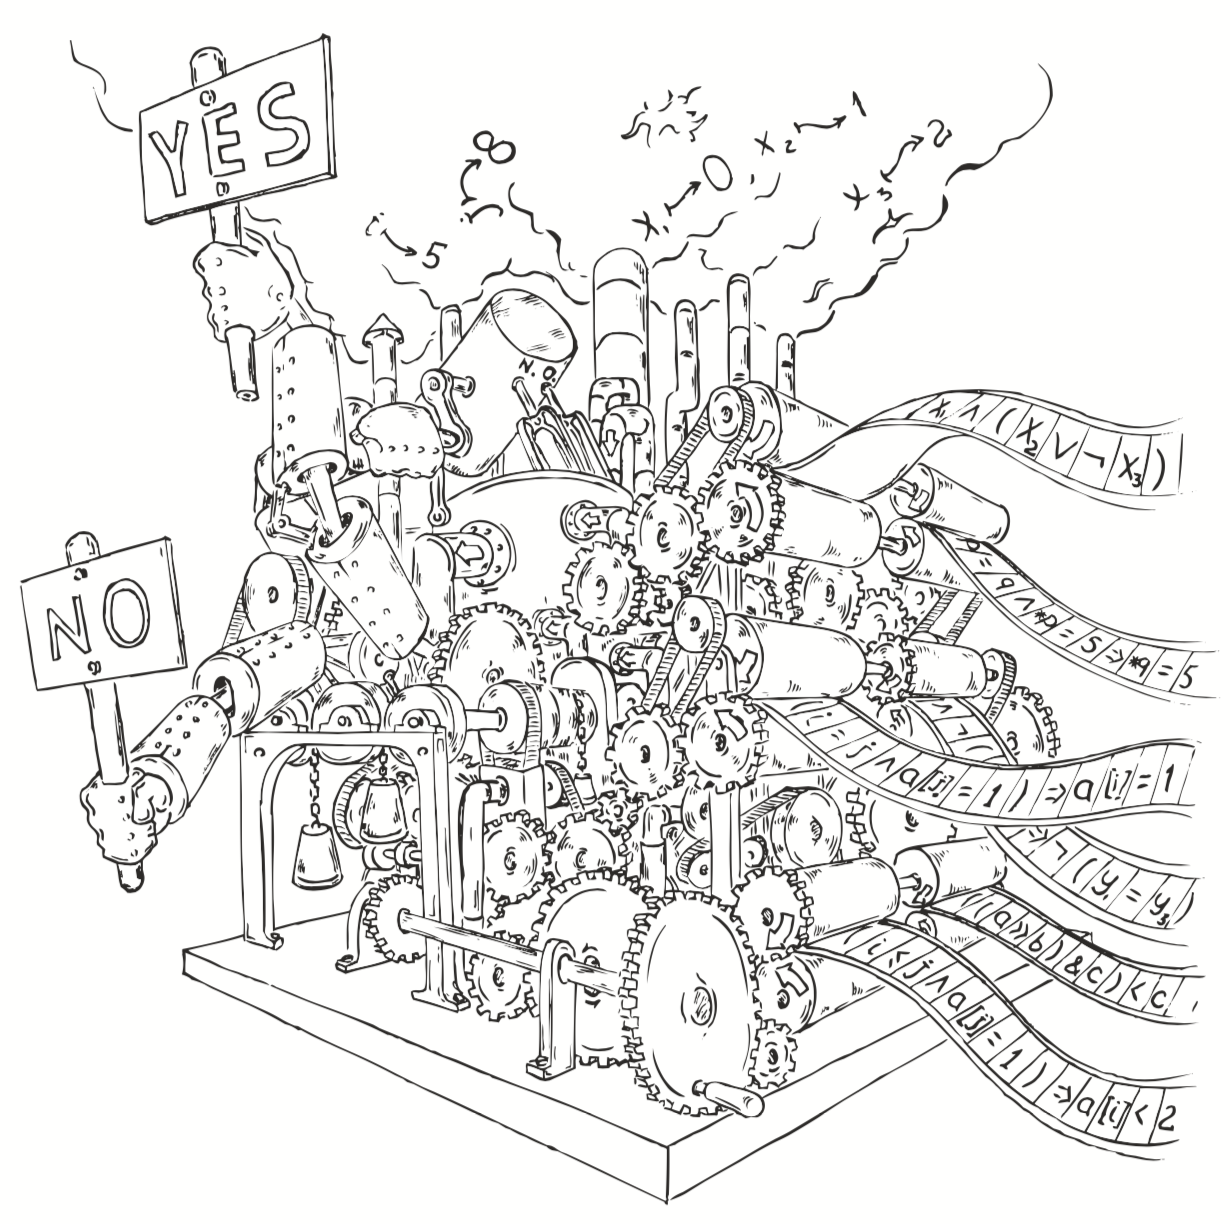
\includegraphics[scale=0.5]{../decision-procedure.png}
\end{frame}

\frame{\titlepage}

\begin{frame}{Пример}
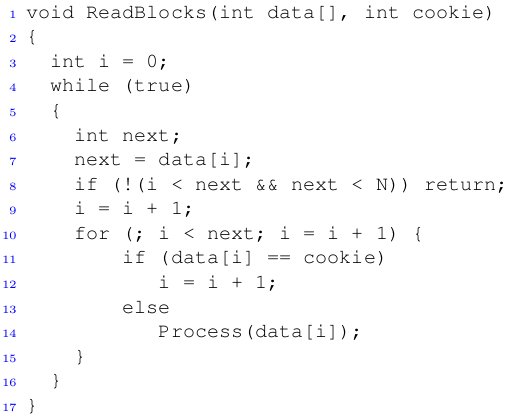
\includegraphics[scale=0.5]{example1.png}
\end{frame}

\begin{frame}{Трасса}
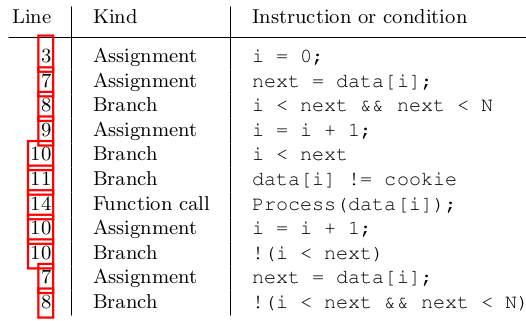
\includegraphics[scale=0.5]{trace1.png}
\end{frame}

\begin{frame}{Static single assignment}
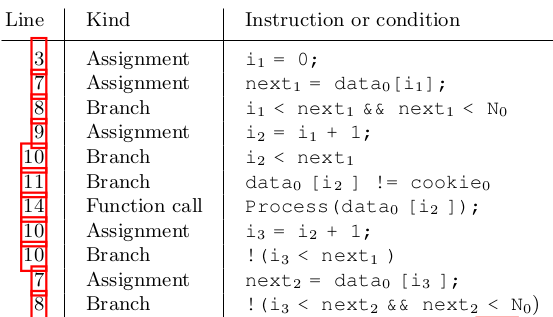
\includegraphics[scale=0.5]{static_single_assignment.png}
\end{frame}

\begin{frame}{Path constraint}
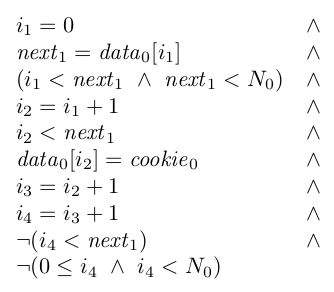
\includegraphics[scale=0.5]{path_constraint1.png}
\end{frame}

\begin{frame}{Пример}
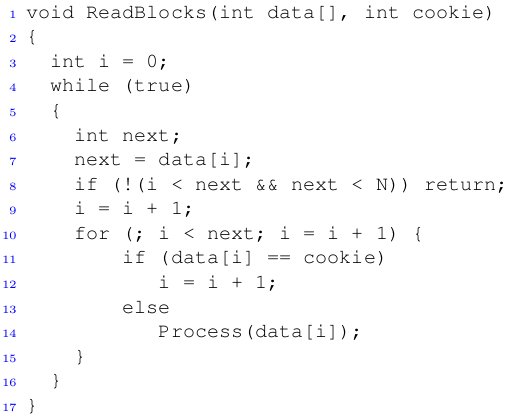
\includegraphics[scale=0.5]{example1.png}
\end{frame}

\begin{frame}{Ошибка}
$i_1 = 0 \wedge \lnot (0 \le i_1 \wedge i_1 < N_0)$\newline
\end{frame}

\begin{frame}{Ошибка}
$i_1 = 0 \wedge \lnot (0 \le i_1 \wedge i_1 < N_0)$\newline
$\{i_1 := 0, N_0 := 0\}$
\end{frame}

\begin{frame}{Другая трасса}
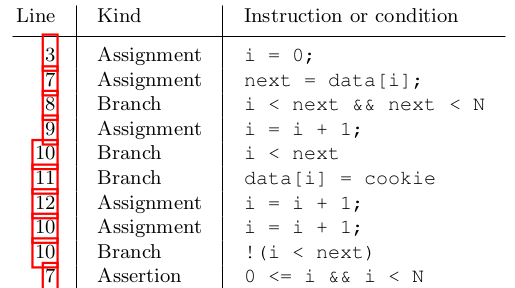
\includegraphics[scale=0.5]{trace2.png}
\end{frame}

\begin{frame}{Path constraint}
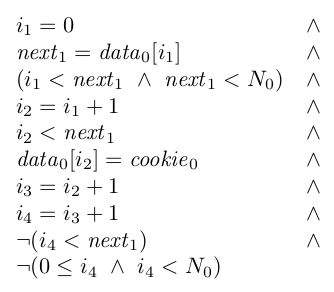
\includegraphics[scale=0.5]{path_constraint2.png}
\end{frame}

\begin{frame}{Оценка входных данных}
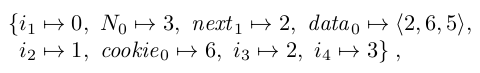
\includegraphics[scale=0.5]{eval.png}
\end{frame}

\begin{frame}{Bounded Program Analysis}
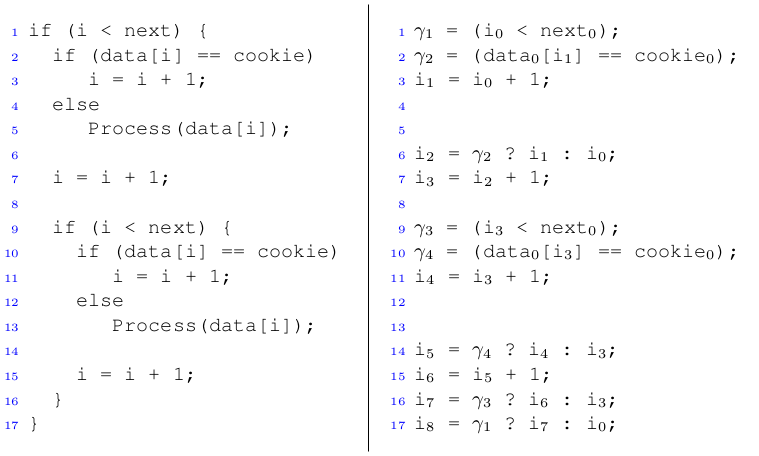
\includegraphics[scale=0.45]{bounded_program_analysis.png}
\end{frame}

\begin{frame}{Unbounded Program Analysis}
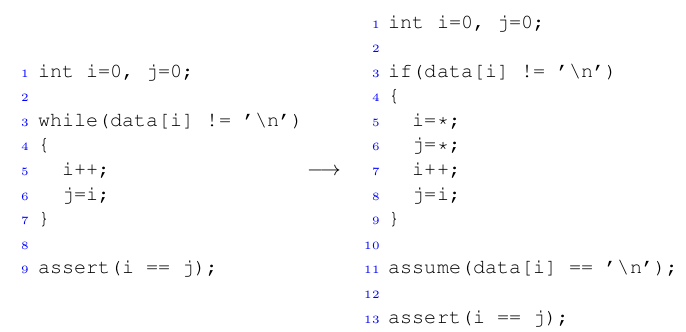
\includegraphics[scale=0.5]{unbounded_program_analysis.png}
\end{frame}

\begin{frame}{Path constraint}
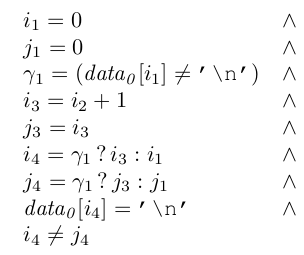
\includegraphics[scale=0.5]{path_constraint3.png}
\end{frame}

\begin{frame}{Неудачный пример аппроксимации}
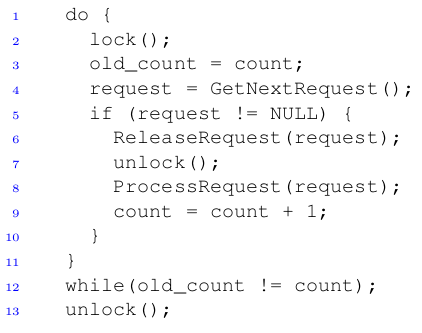
\includegraphics[scale=0.5]{example3.png}
\end{frame}

\begin{frame}{Конечный автомат миханизма взятия лока}
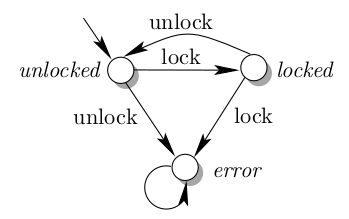
\includegraphics[scale=0.5]{lock_automaton.png}
\end{frame}

\begin{frame}{Добавление assert-ов}
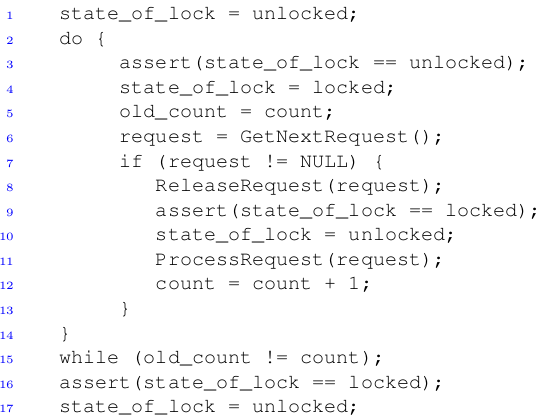
\includegraphics[scale=0.5]{asserts.png}
\end{frame}

\begin{frame}
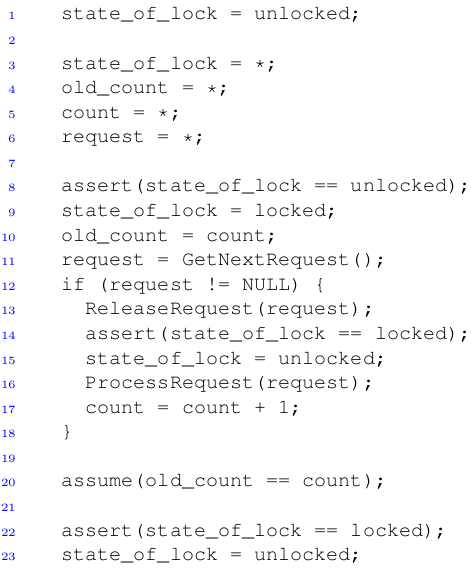
\includegraphics[scale=0.45]{new_code1.png}
\end{frame}

\begin{frame}
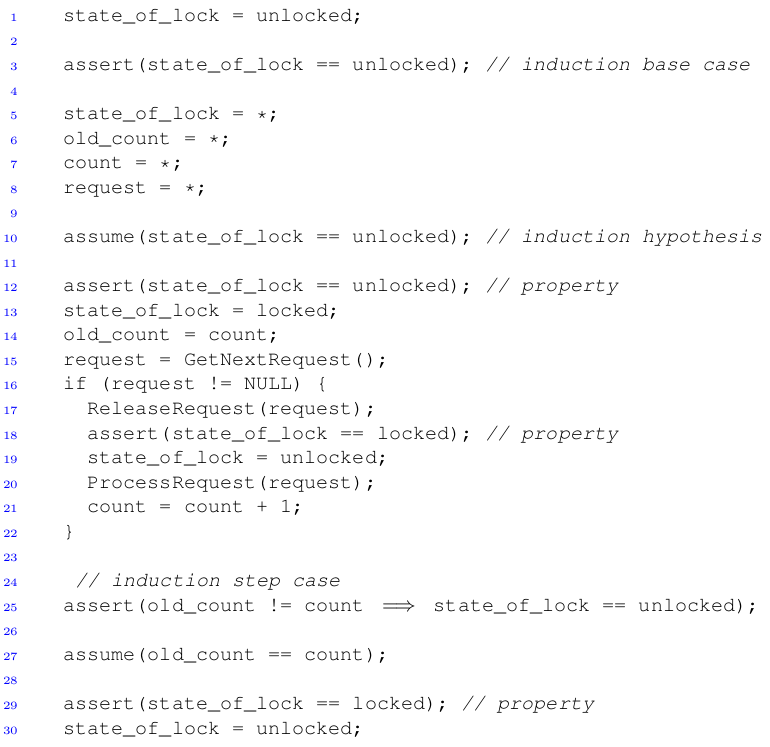
\includegraphics[scale=0.35]{new_code2.png}
\end{frame}

\begin{frame}
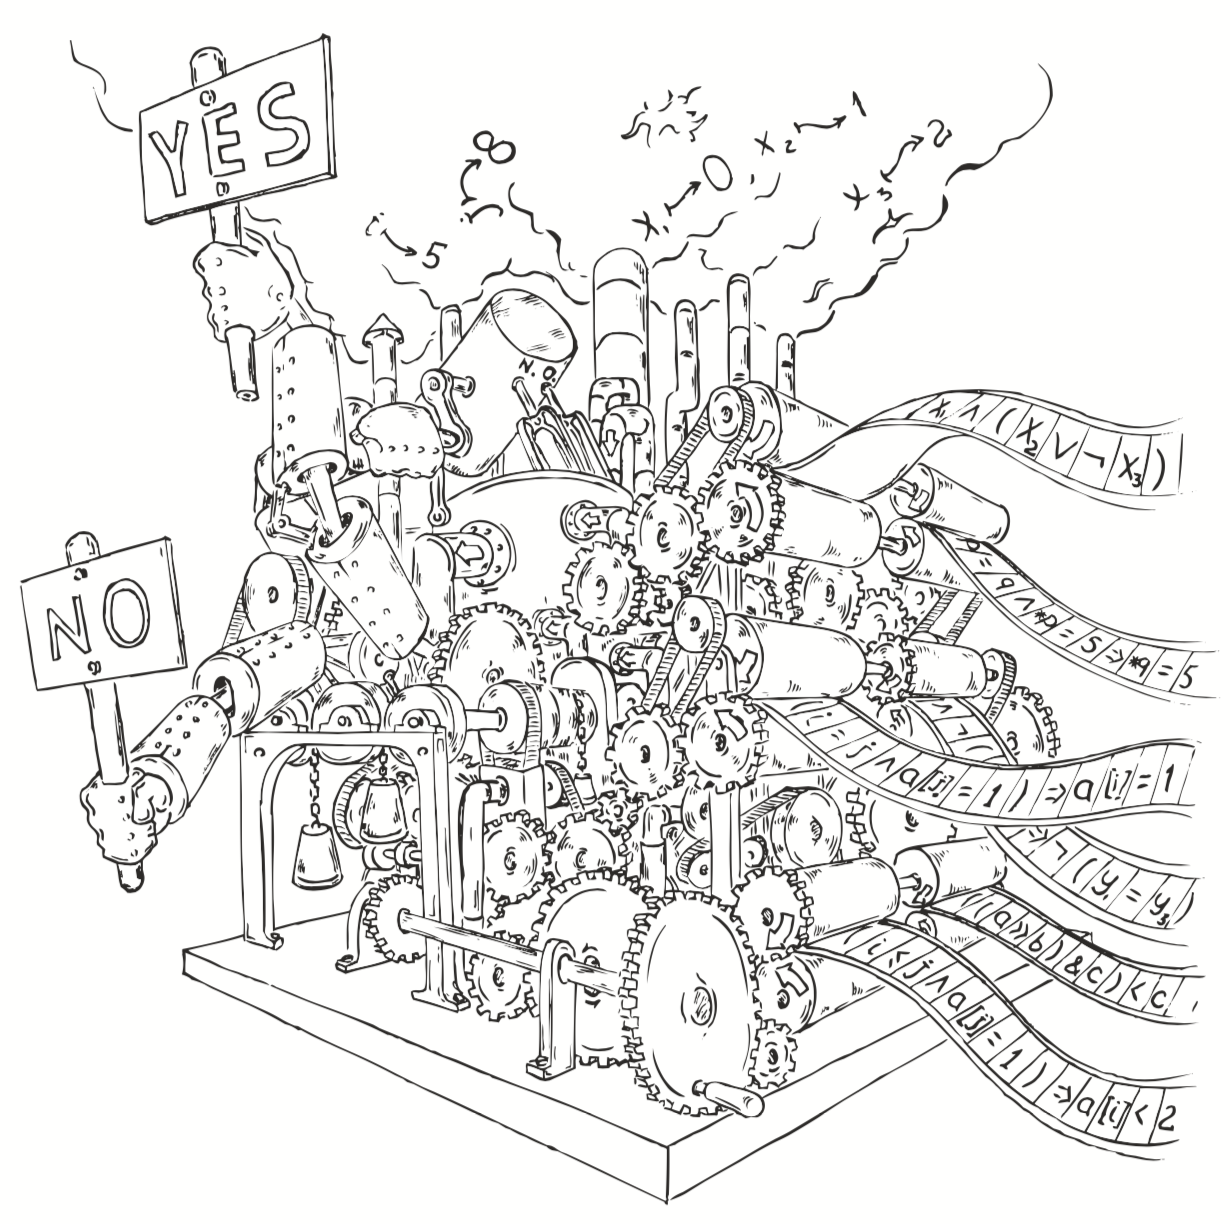
\includegraphics[scale=0.5]{../decision-procedure.png}
\end{frame}

\end{document}
